\subsection*{Learning Objectives}
	Students need to be able to\ldots
	\begin{itemize}
		\item recognize and provide good feedback using the SPARK guidelines.	\end{itemize}

\subsection*{Context}
	This week, students will be providing feedback on their peers' modelling for Homework \#3. As such, there are no problems for students to solve in tutorial.
	

\subsection*{Before Tutorial}

Send an announcement reminding students that they need to bring a draft of Q4 for homework \#3.

\subsection*{What to Do}

	\paragraph{How to provide good feedback (15-20 min)}

	SPARK guidelines.
	
	Essentially, you will be replicating the workshop done in the head TA meetings this week.
	
	Start by asking students what they think makes a piece of feedback good or bad. They can either explain, or give examples. Connect these examples to the SPARK guidelines to explain what makes this feedback good or bad.
	
	If students don't provide any convenient examples, here are the examples of good/bad feedback we saw in this week's workshop:
	\begin{itemize}
		\item ``Everything is perfect!''
		\item ``Your grammar sucks. Did you even use spellcheck?!''
		\item ``You should delete parts of this section from your modelling, you don't need them.''
%		\item ``Your mind map has too many concepts in it. These are good ideas, but the mindmap should be readable without zooming in. I think you should remove at least five of them.''
		\item ``This sentence is very long, which makes it hard to read; you could split it into 3 sentences if you put periods in these places. If you need extra help with writing, your college probably has a writing centre you can use.''
		\item ``I thought it was insightful that you discussed the decline of the lobster fishing industry in your hometown as a reason for exponential population decrease. You've clearly shown your knowledge of your hometown's culture and how it affects the population in mathematical terms.''
	\end{itemize}
	
	The SPARK guidelines are as follows:
	\begin{itemize}
		\item \textbf{Specific:} Comments are linked to a discrete word, phrase, or sentence.
		\item \textbf{Prescriptive:} Prescriptive feedback offers a solution or strategy to improve the work, including possible revisions or links to helpful resources or examples.
		\item \textbf{Actionable:} When the feedback is read, it leaves the peer knowing what steps to take for improvement.
		\item \textbf{Referenced:} The feedback directly references the task criteria, requirements, or target skills.
		\item \textbf{Kind:} It's mandatory that all comments be framed in a kind, supportive way.
	\end{itemize}
	
	

\subsection*{Notes}
	\begin{itemize}
		\item Feedback doesn't need to be critical to be good; positive feedback can also be useful in telling students what to continue doing, as long as it still embodies the SPARK guidelines.
		\item Encourage students to review the feedback that is given to them. If students don't feel that the feedback they receive is useful, they should ask their partner to elaborate.

\end{itemize}
	
	

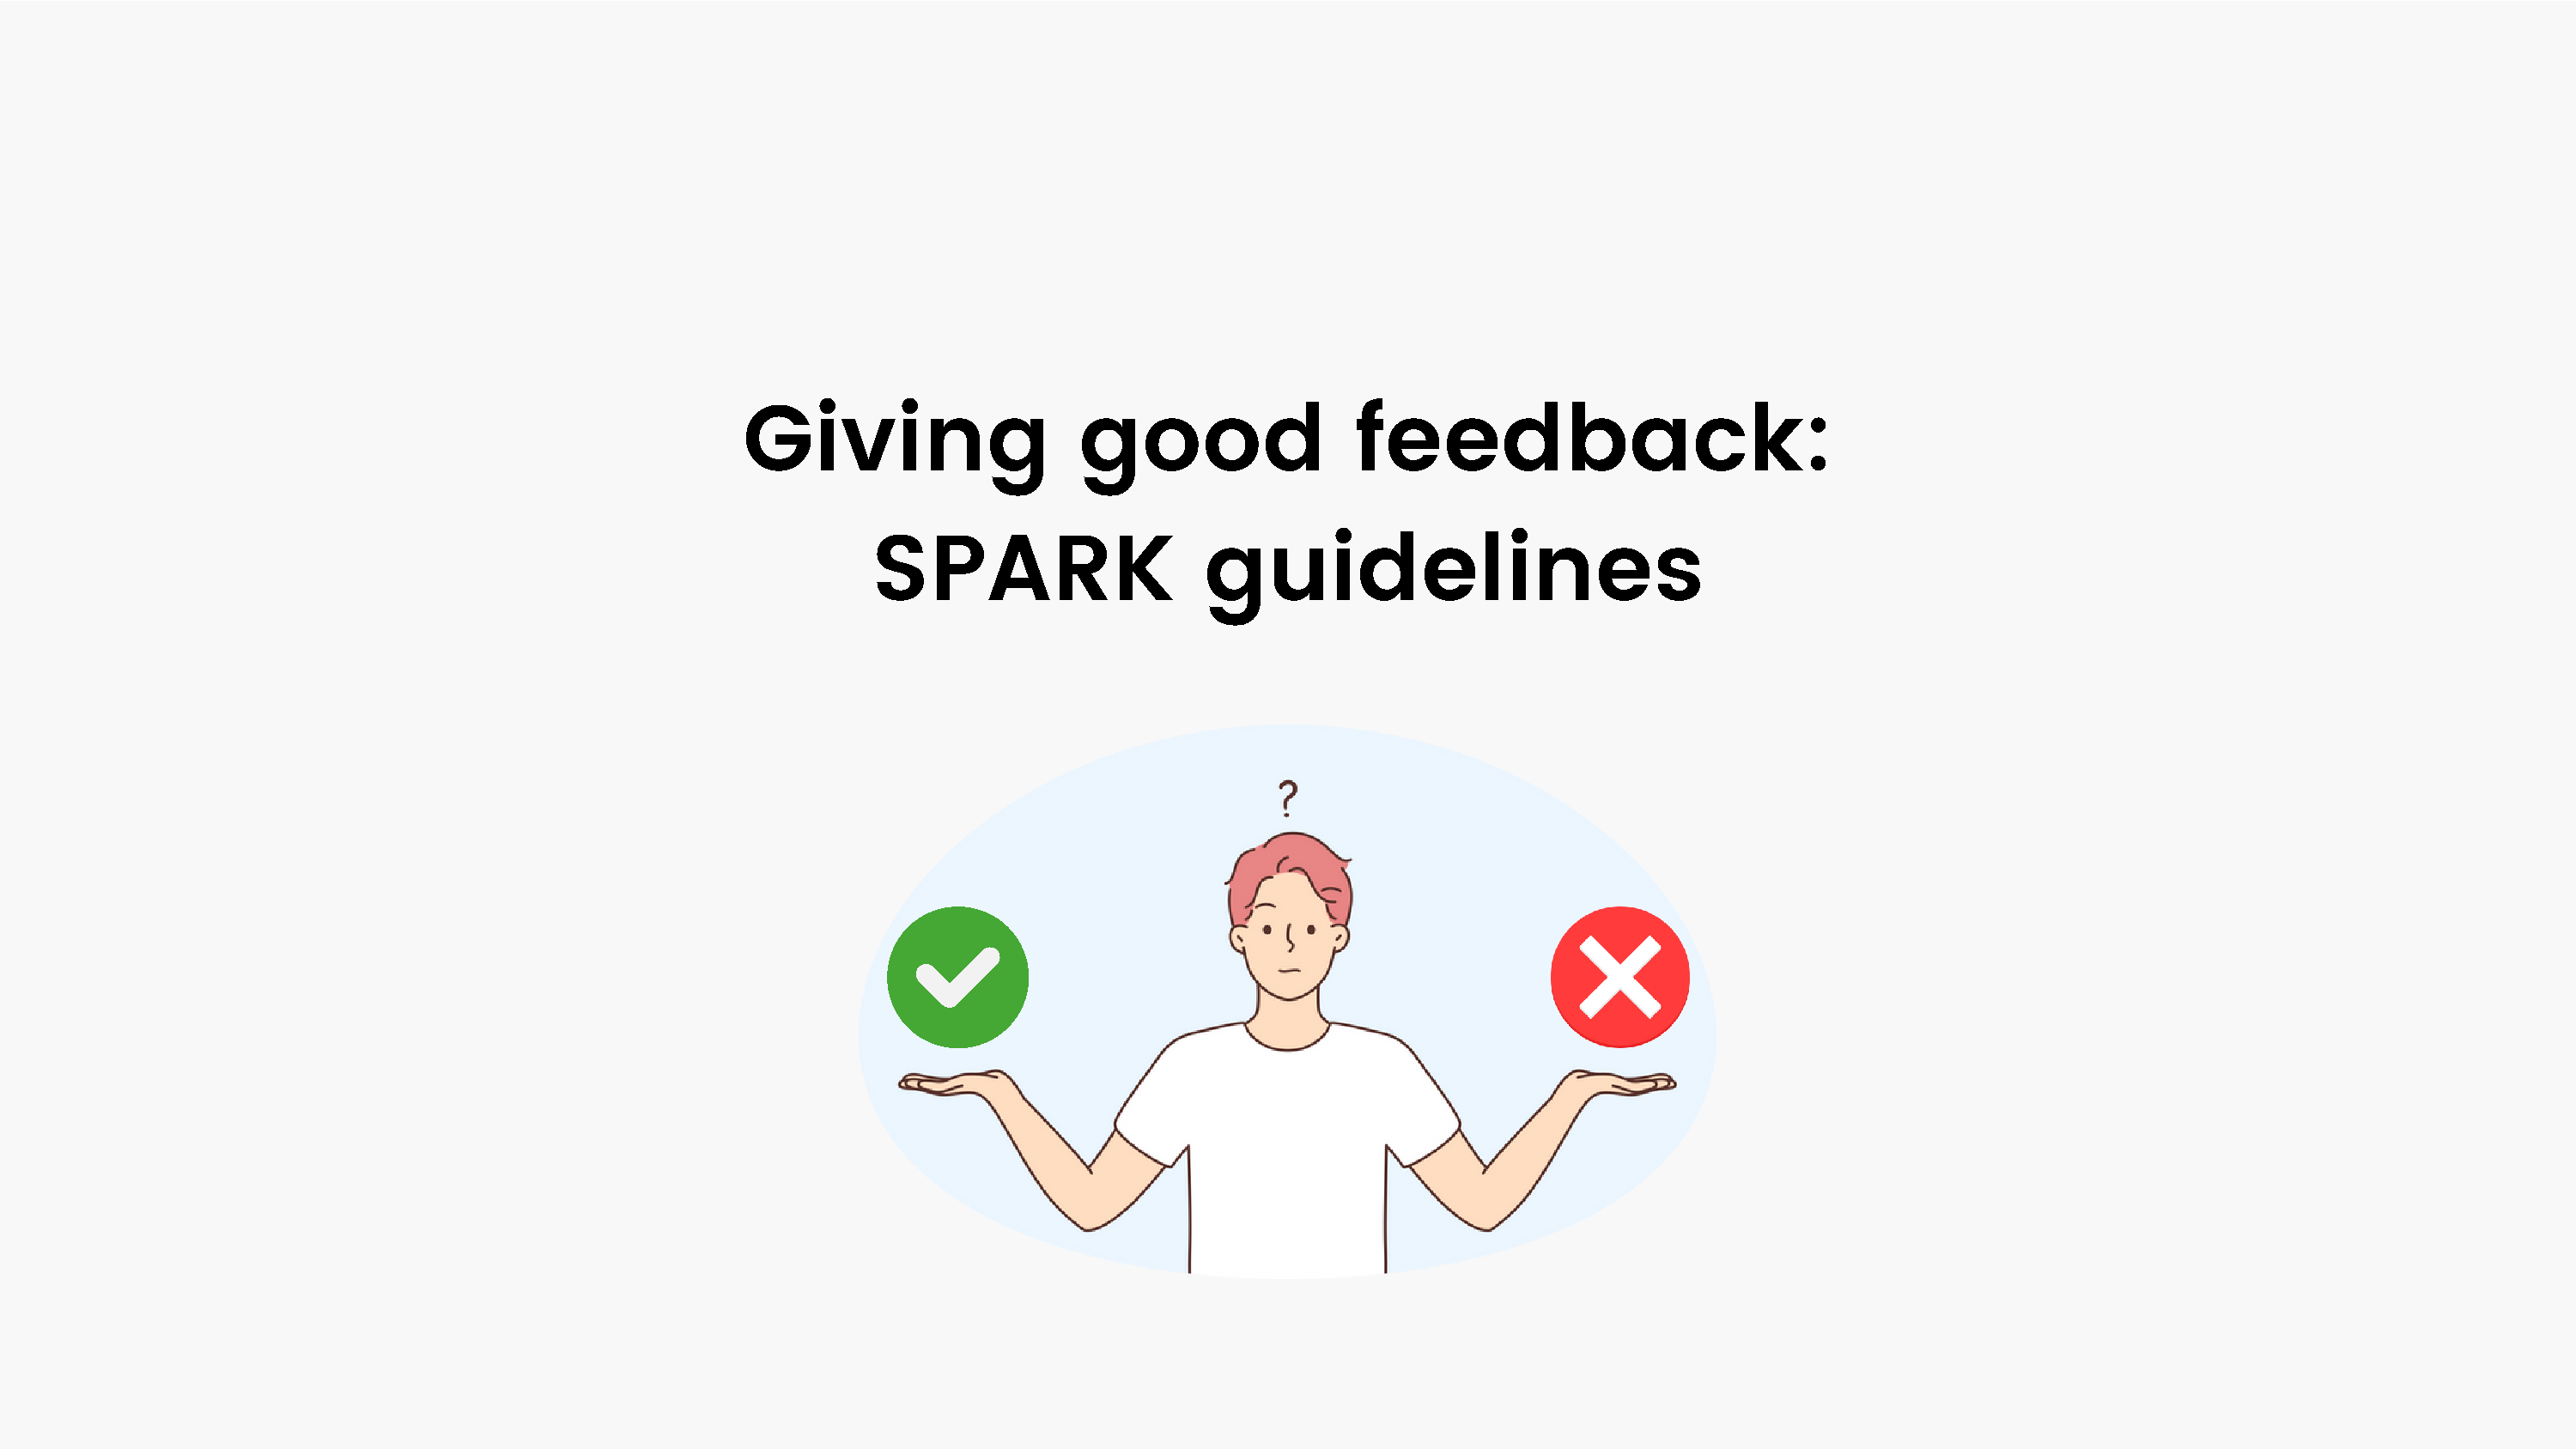
\includegraphics[page=1,width=\textwidth]{resources/tutorial-05-WorkshopFeedbackSPARK.pdf}
\vfil
\includegraphics[page=2,width=\textwidth]{resources/tutorial-05-WorkshopFeedbackSPARK.pdf}
\vfil
\includegraphics[page=3,width=\textwidth]{resources/tutorial-05-WorkshopFeedbackSPARK.pdf}
\vfil
\includegraphics[page=4,width=\textwidth]{resources/tutorial-05-WorkshopFeedbackSPARK.pdf}
\vfil
\includegraphics[page=5,width=\textwidth]{resources/tutorial-05-WorkshopFeedbackSPARK.pdf}
\vfil
\includegraphics[page=6,width=\textwidth]{resources/tutorial-05-WorkshopFeedbackSPARK.pdf}
\vfil
\includegraphics[page=7,width=\textwidth]{resources/tutorial-05-WorkshopFeedbackSPARK.pdf}
\vfil
\includegraphics[page=8,width=\textwidth]{resources/tutorial-05-WorkshopFeedbackSPARK.pdf}


	
	
